\newcommand{\tttt}{Recursie}
\newcommand{\dddd}{Datum 1}

\documentclass{article}
\usepackage[utf8]{inputenc}

\usepackage{listings}
\usepackage{color}
\usepackage{amsmath}
\usepackage{wrapfig}
\usepackage{graphicx}
\graphicspath{ {./images/} }
\usepackage{tikz}

\definecolor{mygreen}{rgb}{0,0.6,0}
\definecolor{mygray}{rgb}{0.5,0.5,0.5}
\definecolor{mymauve}{rgb}{0.58,0,0.82}

\lstset{ %
  backgroundcolor=\color{white},   % choose the background color
  basicstyle=\footnotesize,        % size of fonts used for the code
  breaklines=true,                 % automatic line breaking only at whitespace
  captionpos=b,                    % sets the caption-position to bottom
  commentstyle=\color{mygreen},    % comment style
  escapeinside={\%*}{*)},          % if you want to add LaTeX within your code
  keywordstyle=\color{blue},       % keyword style
  stringstyle=\color{mymauve},     % string literal style
  numbers=left,               % Ort der Zeilennummern
  language=java,
}

\begin{document}

\title{\tttt}
\author{Steven Bronsveld}

\maketitle
\section{Gegevens}
Uiterlijke inleverdatum: \textbf{\dddd}
\subsection{Links}
\begin{itemize}
    \item Github.com/StevenBrons 
    \item https://natureofcode.com/book
    \item http://hello.processing.org/editor/
\end{itemize}


\newpage


\section{Leerdoelen}
\begin{itemize}
    \item Functions met \texttt{return} van type \texttt{int}
    \item Printen naar het console door middel van \texttt{System.out.println()}
    \item Het recursief aanroepen van functions
    \item Het recursief tekenen van simpele fractels
\end{itemize}

\section{Uitleg}
\begin{itemize}
    \item \myhref{https://www.youtube.com/watch?v=-wiverLQl1Q\&list=PLRqwX-V7Uu6bXUJvjnMWGU5SmjhI-OXef\&index=1}{Fractals - The Nature of Code}\\
    Alleen \textbf{8.1, 8.2, 8.3}\\
    \textit{Bij 8.3 wordt er gebruik gemaakt van een \texttt{ArrayList} voor het maken van Koch's Curve. Dit hoef je (nog) niet te kunnen.}
    \item \myhref{https://natureofcode.com/book/chapter-8-fractals/}{Chapter 8. Fractals}\\
    Alleen \textbf{8.1, 8.2, 8.3, 8.4}\\
    \textit{Bij 8.4 wordt er gebruik gemaakt van een \texttt{ArrayList} voor het maken van Koch's Curve. Dit hoef je (nog) niet te kunnen.}
\end{itemize}

\section{Opdrachten}
\subsection{[Optioneel] Recursieve functies}
Recursieve functies zijn functies die een (makkelijkere) versie van zichzelf gebruiken voor het bereken van een antwoord. Kijk bijvoorbeeld naar:
\[f(n) = \begin{cases}
        $1 \qquad\qquad\qquad n = 0$\\
        $3 * f(n-1)  \qquad n $>$ 0$
    \end{cases}
   \]
Deze functie geeft $f(n) = g^n$. Als we dit uitschrijven krijgen we: $f(4) = 3 * f(3) = 3 * 3 * f(2) = 3 * 3 * 3 * f(1) = 3 * 3 * 3 * 3 * f(0) = 3 * 3 * 3 * 3 * 1 = 81 = 3^4$
\[g(n) = \begin{cases}
        $1 \qquad\qquad\qquad n = 0$\\
        $n * g(n-1)  \qquad n $>$ 0$
    \end{cases}
   \]
Schrijf de uitwerking van $g(5)$ helemaal uit. Weet je ook welke functie $g$ is?
\[h(n) = \begin{cases}
        $1 \qquad\qquad\qquad n = 0$\\
        $1 \qquad\qquad\qquad n = 1$\\
        $h(n - 1) + h(n - 2)  \qquad n $>$ 1$
    \end{cases}
   \]
Schrijf de uitwerking van $h(4)$ helemaal uit. Weet je ook welke functie $h$ is?

\subsection{Codeer Koch's Curve}
Vandaag gaan we door middel van \texttt{recursieve functies} fractals tekenen!
In de vorige \textit{assignment} heb je de functie \texttt{kochCurve} geschreven die de figuur \ref{fig:koch} tekent. Als je iedere lijn vervangt door deze zelfde figuur krijg je de situatie van figuur \ref{fig:koch2}. Als je dit oneindig vaak herhaald krijg je een \textbf{fractel} (zie figuur \ref{fig:koch_fract}).
\begin{figure}[H]
	\centering
	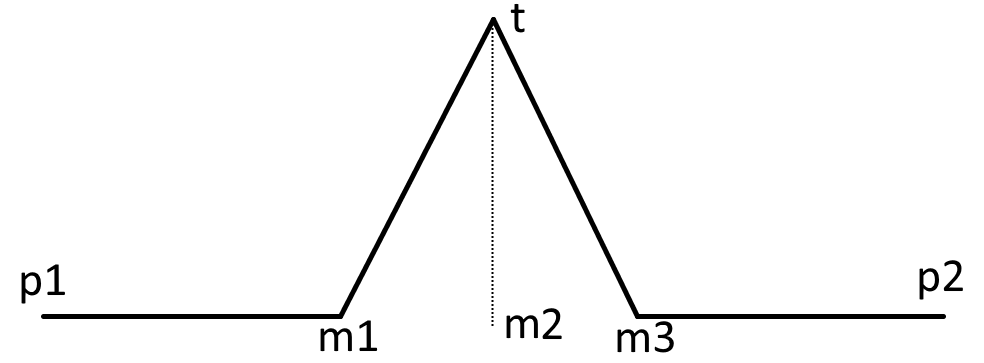
\includegraphics[width=\textwidth]{koch.png}
	\caption{Koch's Curve generatie 1}
	\label{fig:koch}
\end{figure}
\begin{figure}[H]
	\centering
	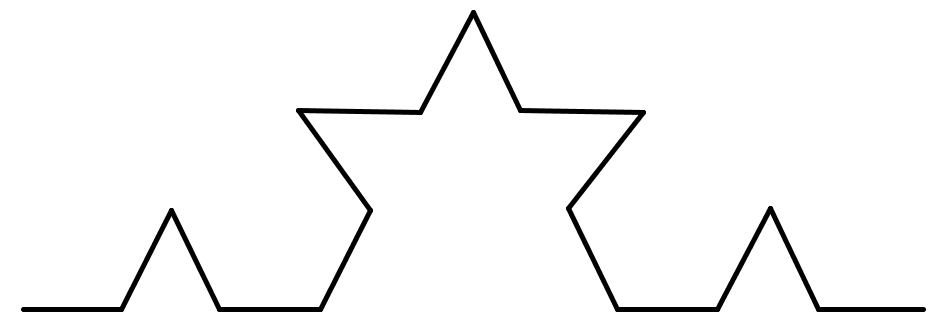
\includegraphics[width=\textwidth]{koch2.png}
	\caption{Koch's Curve generatie 2}
	\label{fig:koch2}
\end{figure}
\begin{figure}[H]
	\centering
	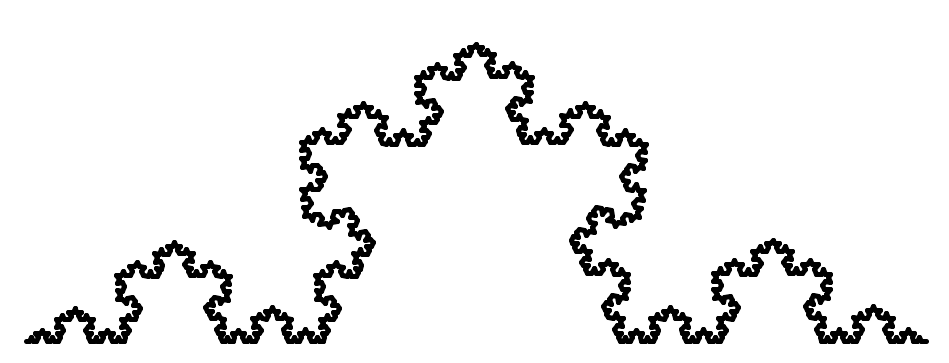
\includegraphics[width=\textwidth]{koch_fract.png}
	\caption{Koch's Curve Fractel (generatie $\infty$)}
	\label{fig:koch_fract}
\end{figure}

In deze opdracht ga je een functie schrijven die dit proces \texttt{n} keer herhaald.\\
Maak gebruik van de al geschreven functie \texttt{kochCurve} van de vorige assignment.
\begin{lstlisting}
void kochCurve(int n,PVector p1, PVector p2) {
    if (n == 0) {
        line(p1.x,p1.y,p2.x,p2.y);
    }else {
        //TODO
    }
}
\end{lstlisting}

\subsection{Codeer een Sierpinski Triangle}

\subsection{Codeer een Binary Tree}
Maak een method
\begin{lstlisting}
void binaryTree(int n,int x, int y) {
}
\end{lstlisting}
Die een \textbf{binary tree} tekent van \texttt{n} diep. Op de co\"ordinaten \texttt{x, y}.



\subsection{[Bonus] Koch's Snowflake}

\subsection{[Bonus] Hilbert's Curve}


\section{Inleveren}
Als je klaar bent met de hele opdracht kun je deze naar je \textit{repository} \texttt{pushen}.



\end{document}
